\documentclass[a4j,fleqn]{jsarticle}

\usepackage{amsmath}
\usepackage{amssymb}
\usepackage{bm}
\usepackage[dvipdfmx]{graphicx, color}
\usepackage{here}
\usepackage{braket}
\usepackage{url}


\renewcommand{\thesection}{問\arabic{section}}
\renewcommand{\thesubsection}{(\arabic{subsection})}


\begin{document}
    \setcounter{page}{8}
    \setcounter{section}{2}
    \section{}
        \subsection{}
        質量$M$(質量数A)の束縛されていない自由な原子核が1個ある状況を考える。この原子核が準位間の遷移によって$\hbar\omega_e0$のエネルギーの$\gamma$線を放射したとする。すると、運動量の保存から原子核は反跳を受けることになる。このときの運動量を$\bm{P}$とすると$P=|\bm{P}|=\frac{1}{c}\hbar\omega_e$であり、反跳後の運動エネルギー$E_R$は
        \begin{eqnarray}
            E_R&&=\frac{P^2}{2M}=\frac{\left(\hbar\omega_e\right)^2}{2Mc^2}=\frac{\hbar\omega_e}{2AM_Nc^2}\hbar\omega_e\,\,\,(M_N=9.4\times10^{2}{\rm[MeV/C^2]}:\text{核子の質量})
        \end{eqnarray}
        となる。準位間のエネルギーを$E$とおくと、$E=\hbar\omega_e+E_R$であり$\hbar\omega_e$と$E$は厳密には等しくないということになる。一方、基底状態にある原子核が$\gamma$線を吸収し励起状態に遷移するときには、$\gamma$線のエネルギー$\hbar\omega_a$に対し、$\hbar\omega_a=E+E_R$となる。\\
         例として、${}^{57}{\rm{Fe}}$の励起状態${}^{57}{\rm{Fe}}^{\ast}$が$14.4{\rm{keV}}$の$\gamma$線を放射し基底状態に遷移する場合を考える。この場合$E_R=2\times10^{-3}{\rm{eV}}$である。この励起状態${}^{57}{\rm{Fe}}^{\ast}$は、以下の図に示すように${}^{57}{\rm{Co}}$が崩壊によって${}^{57}{\rm{Fe}}$を生じた場合に最初にとる状態である。これは$T_{1/2}=9.8\times10^{-8}{\rm{sec}}$の半減期を持ち、基底状態へと遷移する。
        \begin{figure}[H]
            \centering
            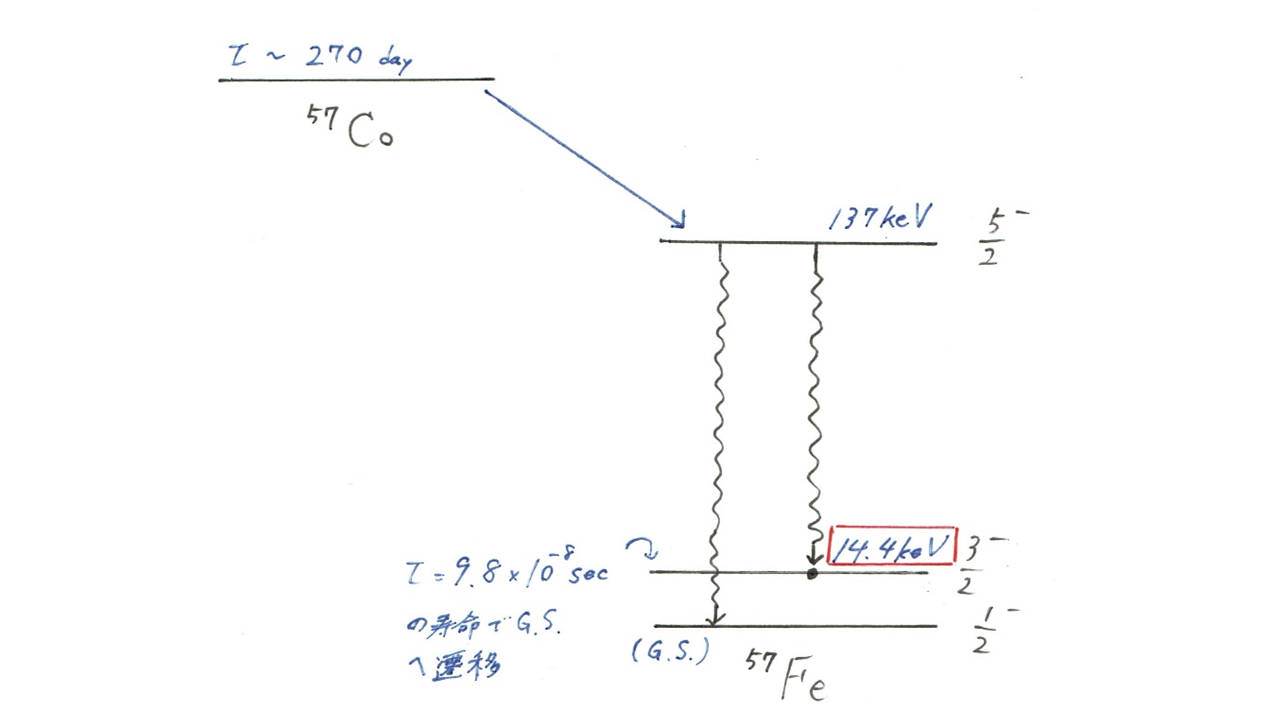
\includegraphics[bb = 0 0 1100 550, width=11.0cm]{tamu_fig04.png}
            \caption{${}^{57}{\rm{Co}}\to{}^{57}{\rm{Fe}}$の準位構造略図}
        \end{figure}
        不確定性原理:$\Gamma\tau\sim\left(\Delta{E}\right)\left(\Delta{t}\right)\sim\hbar$より、この励起状態のエネルギーは
        \begin{eqnarray}
            \Gamma&&\sim\frac{\hbar}{\tau_{{}^{57}{\rm{Fe}}^{\ast}}}=\frac{\hbar{c}\ln{2}}{9.8\times10^{-8}\cdot3\times10^{-7}{\rm[fm]}}=4.7\times10^{-9}{\rm{eV}}
        \end{eqnarray}
        のエネルギー幅$\Gamma$を持つ。このエネルギー幅$\Gamma$は反跳エネルギー$E_R$と比較して6桁ほど小さい値になる。したがって、遷移の際に放射される$\gamma$線と同じエネルギーの$\gamma$線を照射してもこの反跳エネルギー分の消費があるため、基底状態にある${}^{57}{\rm{Fe}}$を再度${}^{57}{\rm{Fe}}^{\ast}$に励起することはできない。\\
         以下では原子核が結晶中の格子点に束縛されている場合を考える。この結晶が$N\sim10^{15}$個(結晶の一般的な粒子数のスケール)の粒子で構成される固体であるとすると、この時の反跳エネルギー$E'_R$は
        \begin{eqnarray}
            E'_R=\frac{\left(\hbar\omega_e\right)^2}{2NM_Nc^2}=10^{-15}E_R&&=2\times10^{-18}{\rm{eV}}<<\frac{1}{2}\Gamma=2.3\times10^{-9}{\rm{eV}}
        \end{eqnarray}
        となる。このように、結晶中にある場合は反跳エネルギーが非常に小さくなる。これは対象の原子核とその周囲の格子点との結合がばねのように働き反跳を吸収するためである。このように通常であれば反跳を伴う$\gamma$線の放出、吸収を反跳を伴わずに引き起こすことができる。特にこれにより基底状態から励起状態への共鳴吸収を引き起こすことができる。このような現象をメスバウアー効果という。\\
         なお、実在の固体は格子の振動数がある値$\omega_D$でカットオフされる。これをDebye振動数とい、これを温度に換算したもの$\Theta_D=\frac{\hbar\omega_D}{k_B}$をDebye温度という。このように格子の振動数に制限があることから、格子点のばね振動によって吸収できる反跳にも限界が存在する。この上限は$\hbar\omega_D=k_B\Theta_D$によって与えられる。ここで、$E_R/k_B\Theta_D$が小さいほど反跳なしの吸収が生じる確率$P$は大きくなる。また、この確率は温度の関数として
        \begin{eqnarray}
            P&&=\exp{\left[-\frac{3E_R}{2k_B\Theta_D}\left\{1+4\left(\frac{T}{\Theta_D}\right)^2\int_{0}^{\frac{\Theta_D}{T}}{{\rm{d}}x\frac{x}{e^x-1}}\right\}\right]}\approx\exp{\left[-\frac{3E_R}{2k_B\Theta_D}\left\{1+\frac{2}{3}\left(\frac{\pi{T}}{\Theta_D}\right)^2\right\}\right]}
        \end{eqnarray}
        のように書くことができる。最後の近似は低温の場合を仮定し、積分範囲を無限大まで拡大したものである。この式から$T$が$\Theta_D$と比較して小さい、即ち低温であるほど確率$P$は増大する。反跳がキャンセルされる上限は、結晶を構成する物質の物性や温度によって決定される。これが既知であれば、共鳴吸収が生じるか生じないかの境界からエネルギー準位幅を決定できる。このことから準位間のエネルギーと準位幅との比をとると、${}^{57}{\rm{Fe}}$の場合には
        \begin{eqnarray}
            \frac{\Gamma}{E}=\frac{4.7\times10^{-9}{\rm{eV}}}{14.4{\rm{keV}}}\sim10^{-13}
        \end{eqnarray}
        となり、非常に高精度でのエネルギーの測定ができるということがわかる。
        \subsection{}
         この実験は1960年にハーバード大学のR.V.PoundとRebkaが地上での重力赤方偏移を測定したものである。彼らは大学内にあった$22.5{\rm{m}}$の高さの塔(Harvard Tower)の下に$\gamma$線として${}^{57}{\rm{Co}}$を、上に${}^{57}{\rm{Fe}}$の吸収体を挟む形で$\gamma$線検出器をそれぞれ設置した。通常ならメスバウアー効果により線源からの$\gamma$線は吸収体の${}^{57}{\rm{Fe}}$によって吸収されてしまうため検出器では検知することができなくなる。ここに重力場の寄与が加えられると、重力赤方偏移によって$\gamma$線の振動数が低くなるため、エネルギーが低くなり${}^{57}{\rm{Fe}}$による吸収は生じず、検出器がこれを感知することになる。そこに吸収体を線源に向かい下向きにゆっくりと動かす操作を加える。このようにすると、ドップラー効果によって青方遷移が生じる。これにより重力場の寄与による赤方偏移を相殺することができるような速さが存在するはずである。もしうまく相殺できれば吸収体で$\gamma$線の共鳴吸収が起こるはずである。そして、もともとの$\gamma$線のエネルギーは既知であるから、この時の速さが分かれば重力赤方偏移を求めることができるのである。
        \begin{figure}[H]
            \centering
            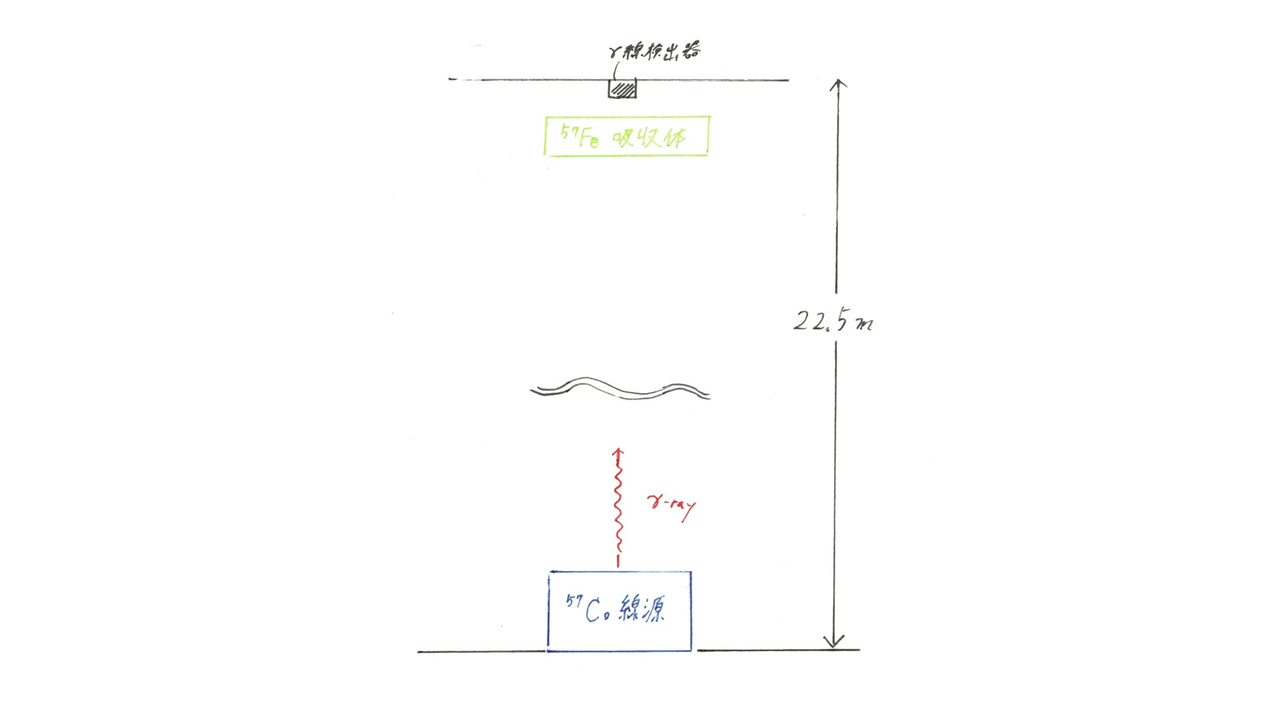
\includegraphics[bb= 0 0 900 550, width=11.0cm]{tamu_fig05.png}
            \caption{Pound-Rebka-Sniderの実験のセットアップ略図}
        \end{figure}
         光のエネルギーの変化は重力場の高次の項を無視する近似の下では次のように求まる。位置$\bm{r}_1$で放出された光が重力に逆らって$\bm{r}_2$に達したとする。位置$\bm{r}_1$及び$\bm{r}_2$での重力ポテンシャルを$\Phi\left(\bm{r}_1\right)$、$\Phi\left(\bm{r}_1\right)$、エネルギーを$\epsilon_{1}$、$\epsilon_{2}$とすると、
        \begin{eqnarray}
            \left\{1+\frac{1}{c^2}\Phi\left(\bm{r}_1\right)\right\}\epsilon_{1}&&=\left\{1+\frac{1}{c^2}\Phi\left(\bm{r}_2\right)\right\}\epsilon_{2}\\
            \epsilon_{2}&&=\left\{1+\frac{1}{c^2}\Phi\left(\bm{r}_2\right)\right\}^{-1}\left\{1+\frac{1}{c^2}\Phi\left(\bm{r}_1\right)\right\}\epsilon_{1}\\
            &&\sim\left\{1-\frac{1}{c^2}\Phi\left(\bm{r}_2\right)\right\}\left\{1+\frac{1}{c^2}\Phi\left(\bm{r}_1\right)\right\}\epsilon_{1}\\
            &&\sim\left[1+\frac{1}{c^2}\left\{\Phi\left(\bm{r}_1\right)-\Phi\left(\bm{r}_2\right)\right\}\right]\epsilon_1\\
            \therefore\Delta\epsilon\equiv&&\epsilon_2-\epsilon_1\sim\frac{1}{c^2}\left\{\Phi\left(\bm{r}_1\right)-\Phi\left(\bm{r}_2\right)\right\}\epsilon_1
        \end{eqnarray}
        と書ける。\\
         このことから塔の高さ:22.5mで期待されるエネルギーの変化分$\Delta{E}$は
        \begin{eqnarray}
            \Delta{E}&&=mgh=\frac{1}{c^2}Egh=\frac{14.4{\rm{keV}}}{c^2}\cdot9.8{\rm{m/s^{-2}}}\cdot22.5{\rm{m}}=3.5\times10^{-11}{\rm{eV}}
        \end{eqnarray}
        である。これと元のエネルギー$E$との比を取った値は
        \begin{eqnarray}
            \frac{\Delta{E}}{E}=\frac{2\cdot3.5\times10^{-11}{\rm{eV}}}{14.4{\rm{keV}}}=4.9\times10^{-15}
        \end{eqnarray}
        となる。これが実験において期待される値であった。実際の測定では$5.13\left(\pm0.51\right)10^{-15}$という値が得られた。理論値と実測値との比は$1.05\pm0.10$であった。その5年後の1965年にはR.V.PoundとJ.L.Sniderがより精度を向上させた実験を行った。この時には理論値と実測値との比として$0.9990\pm0.0076$という値を得た。このようにメスバウアー効果を用いた実験によって1パーセントほどの精度で理論値と一致する結果が得られている。\\
        \newpage
        \textbf{問3の参考文献・URL}
        \begin{description}
            \item[(1)-1.]八木浩輔: 基礎物理科学シリーズ4 原子核物理学 (朝倉書店)
            \item[(1)-2.]中嶋貞雄、豊沢豊、阿部龍蔵: 現代物理学の基礎7 物性II 素励起の物理 (岩波書店)
            \item[(2)-1.]\url{https://tenkyo.net/kaiho/pdf/2002_05/2002-05-09.pdf}
            \item[(2)-2.]\url{http://www.icrr.u-tokyo.ac.jp/ss/2014data/lecture/ohashi.pdf}
            \item[(2)-3.] 相対論II(服部誠先生担当)の講義資料\\\url{https://www.astr.tohoku.ac.jp/~hattori/Relativity.pdf}
        \end{description}
        (URLはいずれも2019年8月8日閲覧)
        \newpage
    \section{}
        \subsection{}
        \textbf{(i).電荷分布一様の時}\\
        まず、電荷密度分布が一様である場合を考える。この場合、電荷密度$\rho(\bm{r})$は以下のように書ける。
        \begin{eqnarray}
            \rho(\bm{r})=\frac{Ze}{\frac{4\pi}{3}R^3}\theta(r-R)=
            \begin{cases}
                \frac{3Ze}{4\pi{R^3}}&:r<R\\
                0&:r>R
            \end{cases}
        \end{eqnarray}
        この時、平均2乗半径$\left<r^2\right>$は以下のように計算される。
        \begin{eqnarray}
            \left<r^2\right>&&=\frac{\int_{0}^{+\infty}{r^2\rho(\bm{r})4\pi{r^2}dr}}{\int_{0}^{+\infty}{\rho(\bm{r})4\pi{r^2}dr}}\\
            &&=\frac{\int_{0}^{R}{r^2\left(\frac{3Ze}{4\pi{R^3}}\right)4\pi{r^2}dr}}{\int_{0}^{R}{\left(\frac{3Ze}{4\pi{R^3}}\right)4\pi{r^2}dr}}\\
            &&=\frac{\int_{0}^{R}{r^4dr}}{\int_{0}^{R}{r^2dr}}\\
            &&=\frac{\frac{1}{5}r^5\bigg|_{0}^{R}}{\frac{1}{3}r^3\bigg|_{0}^{R}}\\
            &&=\frac{3}{5}R^2\,\,\,\,\,\,\,\therefore\left<r^2\right>=\frac{3}{5}R^2
        \end{eqnarray}
        \textbf{(ii).電荷分布がガウス分布の時}\\
        次に、電荷分布が標準偏差$\sigma$のGauss分布に従う場合を考える。分布関数は、無限遠まで含めた3次元空間における積分が$1$に規格化されなければならないという条件から、以下のようになる。
        \begin{eqnarray}
            \rho\left(r\right)&&=\frac{Ze}{\left(2\pi\sigma^2\right)^{\frac{3}{2}}}\exp{\left(-\frac{1}{2\sigma^2}r^2\right)}
        \end{eqnarray}
        この時、平均2乗半径は以下のようになる。
        \begin{eqnarray}
            \left<r^2\right>&&=\frac{\int_{0}^{+\infty}{r^2\rho(\bm{r})4\pi{r^2}dr}}{\int_{0}^{+\infty}{\rho(\bm{r})4\pi{r^2}dr}}=\frac{\int_{0}^{+\infty}{r^4\exp{\left(-\frac{1}{2\sigma^2}r^2\right)}dr}}{\int_{0}^{+\infty}{{r^2}\exp{\left(-\frac{1}{2\sigma^2}r^2\right)}dr}}
        \end{eqnarray}
        この積分を実行するにあたり、次のような積分$I_n\left(\alpha\right)$の値を考える。
        \begin{eqnarray}
            I_n\left(\alpha\right)&&\equiv\int_{0}^{+\infty}{dr{r^{2n}\exp{\left(-\alpha{r^2}\right)}}}
        \end{eqnarray}
        但し、$n=0$のときには
        \begin{eqnarray}
            I_0\left(\alpha\right)&&=\int_{0}^{+\infty}{dr{\exp{\left(-\alpha{r^2}\right)}}}=\frac{1}{2}\int_{-\infty}^{+\infty}{dr{\exp{\left(-\alpha{r^2}\right)}}}=\frac{1}{2}\sqrt{\frac{\pi}{\alpha}}
        \end{eqnarray}
        である。ここで、ガウス分布関数の微分に関して、
        \begin{eqnarray}
            &&\frac{{\rm{d}}}{{\rm{d}}r}\exp{\left(-\alpha{r^2}\right)}=-2\alpha{r}\exp{\left(-\alpha{r^2}\right)}\,\,\,\Rightarrow{r}\exp{\left(-\alpha{r^2}\right)}=-\frac{1}{2\alpha}\frac{{\rm{d}}}{{\rm{d}}r}\exp{\left(-\alpha{r^2}\right)}
        \end{eqnarray}
        となることを用いれば、
        \begin{eqnarray}
            I_n\left(\alpha\right)&&=\int_{0}^{+\infty}{dr\left[r^{2n-1}\left(-\frac{1}{2\alpha}\right)\frac{{\rm{d}}}{{\rm{d}}r}\exp{\left(-\alpha{r^2}\right)}\right]}\\
            &&=-\frac{1}{2\alpha}r^{2n-1}\exp{\left(-\alpha{r^2}\right)}\Bigg|_{0}^{+\infty}+\frac{2n-1}{2\alpha}\int_{0}^{+\infty}{dr{r^{2\left(n-1\right)}\exp{\left(-\alpha{r^2}\right)}}}\\
            &&=\frac{2n-1}{2\alpha}I_{n-1}\left(\alpha\right)
        \end{eqnarray}
        これにより、$I_n\left(\alpha\right)$は
        \begin{eqnarray}
            I_n\left(\alpha\right)&&=\frac{2n-1}{\alpha}I_{n-1}\left(\alpha\right)=\frac{2n-1}{2\alpha}\cdot\frac{2n-3}{2\alpha}I_{n-2}\left(\alpha\right)=\cdots=\frac{\left(2n-1\right)!!}{2^n\alpha^n}I_0\left(\alpha\right)=\frac{\left(2n-1\right)!!}{2^{n+1}\alpha^n}\sqrt{\frac{\pi}{\alpha}}
        \end{eqnarray}
        これを利用すれば平均2乗半径の計算は次のようになる。
        \begin{eqnarray}
            \left<r^2\right>&&=\frac{\int_{0}^{+\infty}{r^4\exp{\left(-\frac{1}{2\sigma^2}r^2\right)}dr}}{\int_{0}^{+\infty}{{r^2}\exp{\left(-\frac{1}{2\sigma^2}r^2\right)}dr}}\\
            &&=\frac{I_{2}\left(\frac{1}{2\sigma^2}\right)}{I_{1}\left(\frac{1}{2\sigma^2}\right)}\\
            &&=\frac{\frac{3!!}{2^3}\left(2\sigma^2\right)^2}{\frac{2\sigma^2}{2^2}}\\
            &&=3\sigma^2
        \end{eqnarray}
        両者の分布で$\left<r^2\right>$の値が等しくなるように$\sigma$の値を決定するとすれば、
        \begin{eqnarray}
            3\sigma^2&&=\frac{3}{5}R^2\,\,\,\therefore\sigma=\frac{1}{\sqrt{5}}R
        \end{eqnarray}
        \subsection{}
        標的が原子核等の内部構造を持つ複合粒子である場合には、$E$:入射粒子のエネルギー、$\theta$:散乱角、$k$:運動量移行とすると、微分断面積は以下のように書ける。
        \begin{eqnarray}
            \frac{d\sigma}{d\Omega}&&=\left(\frac{Ze^2}{2E}\right)^2\frac{\cos^2{\frac{\theta}{2}}}{\sin^4{\frac{\theta}{2}}}\left|F(\bm{k})\right|^2
        \end{eqnarray}
        ここで$F(\bm{k})$は電荷密度$\rho\left(\bm{r}\right)$のFourier変換である。
        \begin{eqnarray}
            F(\bm{k})&&=\int{{\rm{d}}^3\bm{r}{\rho\left(\bm{r}\right)e^{i\bm{k}\cdot\bm{r}}}}=4\pi\int_{0}^{+\infty}{r^2\rho\left(\bm{r}\right)\frac{\sin{kr}}{kr}{\rm{d}}r}
        \end{eqnarray}
        \textbf{(i).電荷分布一様の時}\\
         この時の$F(\bm{k})$は以下のようになる。
        \begin{eqnarray}
            F(\bm{k})&&=4\pi\int_{0}^{R}{\left(\frac{3Ze}{4\pi{R^3}}\right)r^2\frac{\sin{kr}}{kr}{\rm{d}}r}\\
            \nonumber&&=4\pi\cdot\frac{3Ze}{4\pi{R^3}}\int_{0}^{R}{\frac{r}{k}\sin{kr}{\rm{d}}r}\\
            \nonumber&&=\frac{3Ze}{R^3}\cdot\frac{1}{k}\int_{0}^{R}{r\sin{kr}{\rm{d}}r}\\
            \nonumber&&=\frac{3Ze}{kR^3}\left[-\frac{r}{k}\cos{kr}\bigg|_{0}^{R}+\frac{1}{k}\int_{0}^{R}{\cos{kr}{\rm{d}}r}\right]\\
            \nonumber&&=\frac{3Ze}{kR^3}\left[-\frac{R}{k}\cos{kR}+\frac{1}{k^2}\sin{kR}\right]\\
            \nonumber&&=\frac{3Ze}{k^3R^3}\left[\sin{kR}-{kR}\cos{kR}\right]\\
            \nonumber\therefore\left|F(\bm{k})\right|^2&&=\left(\frac{3Ze}{k^3R^3}\right)^2\left|\sin^2{kR}-2{kR}\sin{kR}\cos{kR}+\left(kR\right)^2\cos^2{kR}\right|\\
            \nonumber&&=\left(\frac{3Ze}{k^3R^3}\right)^2\left|\sin^2{kR}+\cos^2{kR}-{kR}\sin{2kR}+\left\{\left(kR\right)^2-1\right\}\cos^2{kR}\right|\\
            \nonumber&&=\left(\frac{3Ze}{k^3R^3}\right)^2\left|1-{kR}\sin{2kR}+\frac{1}{2}\left\{\left(kR\right)^2-1\right\}\left(1+\cos{2kR}\right)\right|\\
            \nonumber&&=\left(\frac{3Ze}{k^3R^3}\right)^2\left|\frac{1}{2}\left\{\left(kR\right)^2+1\right\}+\frac{1}{2}\left\{\left(kR\right)^2-1\right\}\cos{\left(2kR\right)}-{kR}\sin{\left(2kR\right)}\right|
        \end{eqnarray}
        したがって、微分断面積は運動量移行:$k$の関数として以下のようになる。
        \begin{eqnarray}
            \frac{d\sigma}{d\Omega}&&=\left(\frac{Ze^2}{2E}\right)^2\frac{\cos^2{\frac{\theta}{2}}}{\sin^4{\frac{\theta}{2}}}\left|F(\bm{k})\right|^2\\
            &&=\frac{1}{4E^2}\frac{9Z^4e^6}{k^6R^6}\frac{\cos^2{\frac{\theta}{2}}}{\sin^4{\frac{\theta}{2}}}\left|\frac{1}{2}\left\{\left(kR\right)^2+1\right\}+\frac{1}{2}\left\{\left(kR\right)^2-1\right\}\cos{\left(2kR\right)}-{kR}\sin{\left(2kR\right)}\right|
        \end{eqnarray}
        \textbf{(ii).電荷分布がガウス分布の時}\\
         この場合の形状因子$F(\bm{k})$は次のように計算される。
        \begin{eqnarray}
            F\left(\bm{k}\right)&&=4\pi\int_{0}^{+\infty}{\frac{Ze}{\left(2\pi\sigma^2\right)^{\frac{3}{2}}}\exp{\left(-\frac{1}{2\sigma^2}r^2\right)}r^2\frac{\sin{kr}}{kr}{\rm{d}}r}\\
            \nonumber&&=\frac{Ze}{k\left(2\pi\sigma^2\right)^{\frac{3}{2}}}\int_{0}^{+\infty}{\exp{\left(-\frac{1}{2\sigma^2}r^2\right)}r{\sin{kr}}{\rm{d}}r}\\
            \nonumber&&=\frac{Ze}{2k\left(2\pi\sigma^2\right)^{\frac{3}{2}}}\int_{-\infty}^{+\infty}{\exp{\left(-\frac{1}{2\sigma^2}r^2\right)}r{\sin{kr}}{\rm{d}}r}\,\,\,\left(\because\text{被積分関数が偶関数であることから積分範囲を拡大}\right)\\
            \nonumber&&=\frac{Ze}{2k\left(2\pi\sigma^2\right)^{\frac{3}{2}}}\int_{-\infty}^{+\infty}{{\sin{kr}}\left(-\sigma^2\right)\frac{{\rm{d}}}{{\rm{d}}r}\exp{\left(-\frac{1}{2\sigma^2}r^2\right)}{\rm{d}}r}\\
            \nonumber&&=\frac{Ze}{2k\left(2\pi\sigma^2\right)^{\frac{3}{2}}}\left[\left(-\sigma^2\right){\sin{kr}}\exp{\left(-\frac{1}{2\sigma^2}r^2\right)}\Bigg|_{-\infty}^{+\infty}-\left(-\sigma^2\right)\int_{-\infty}^{+\infty}{\exp{\left(-\frac{1}{2\sigma^2}r^2\right)}{k\cos{kr}}{\rm{d}}r}\right]
        \end{eqnarray}
        \begin{eqnarray}
            \nonumber&&=\frac{Ze}{2k\left(2\pi\sigma^2\right)^{\frac{3}{2}}}\sigma^2k\int_{-\infty}^{+\infty}{\exp{\left(-\frac{1}{2\sigma^2}r^2\right)}{\frac{1}{2}\left(e^{ikr}+e^{-ikr}\right)}{\rm{d}}r}\\
            \nonumber&&=\frac{Ze}{2k\left(2\pi\sigma^2\right)^{\frac{3}{2}}}\frac{1}{2}\sigma^2k\int_{-\infty}^{+\infty}{\left[\exp{\left(-\frac{1}{2\sigma^2}r^2+ikr\right)}+\exp{\left(-\frac{1}{2\sigma^2}r^2-ikr\right)}\right]{\rm{d}}r}
        \end{eqnarray}
        \begin{eqnarray}
            -\frac{1}{2\sigma^2}r^2\pm{ikr}&&=-\frac{1}{2\sigma^2}\left(r^2\pm2i\sigma^2kr\right)\\
            &&=-\frac{1}{2\sigma^2}\left\{\left(r^2\pm{i\sigma^2k}\right)-\left(i\sigma^2k\right)^2\right\}\\
            &&=-\frac{1}{2\sigma^2}\left(r\pm{i\sigma^2k}\right)^2-\frac{1}{2\sigma^2}\sigma^4k^2\\
            &&=-\frac{1}{2\sigma^2}\left(r\pm{i\sigma^2k}\right)^2-\frac{1}{2}\sigma^2k^2
        \end{eqnarray}
        であることを用いれば、
        \begin{eqnarray}
            \nonumber&&\cdots=\frac{Ze}{2k\left(2\pi\sigma^2\right)^{\frac{3}{2}}}\frac{1}{2}\sigma^2k\int_{-\infty}^{+\infty}{{\rm{d}}r\exp{\left(-\frac{1}{2}\sigma^2k^2\right)}\left[\exp{\left\{-\frac{1}{2\sigma^2}\left(r-{i\sigma^2k}\right)^2\right\}}+\exp{\left\{-\frac{1}{2\sigma^2}\left(r+{i\sigma^2k}\right)^2\right\}}\right]}\\
            \nonumber&&=\frac{Ze}{2k\left(2\pi\sigma^2\right)^{\frac{3}{2}}}\frac{1}{2}\sigma^2k\exp{\left(-\frac{1}{2}\sigma^2k^2\right)}2\sqrt{2\pi\sigma^2}\\
            &&=\frac{Ze}{4\pi}\exp{\left(-\frac{1}{2}\sigma^2k^2\right)}
        \end{eqnarray}
        これにより、
        \begin{eqnarray}
            \frac{d\sigma}{d\Omega}&&=\left(\frac{Ze^2}{2E}\right)^2\frac{\cos^2{\frac{\theta}{2}}}{\sin^4{\frac{\theta}{2}}}\left|F(\bm{k})\right|^2\\
            &&=\left(\frac{Ze^2}{2E}\right)^2\frac{\cos^2{\frac{\theta}{2}}}{\sin^4{\frac{\theta}{2}}}\left(\frac{Ze}{4\pi}\right)^2\exp{\left(-\sigma^2k^2\right)}\\
            &&=\frac{Z^4e^6}{64\pi^2E^2}\frac{\cos^2{\frac{\theta}{2}}}{\sin^4{\frac{\theta}{2}}}\exp{\left(-\sigma^2k^2\right)}
        \end{eqnarray}
        である。これに、前問(1)で求めた$\sigma$と$R$の関係を代入すると、最終的に電荷分布がガウス分布であるときの微分断面積は以下のようになる。
        \begin{eqnarray}
            \frac{d\sigma}{d\Omega}&&=\frac{Z^4e^6}{64\pi^2E^2}\frac{\cos^2{\frac{\theta}{2}}}{\sin^4{\frac{\theta}{2}}}\exp{\left(-\frac{1}{5}k^2R^2\right)}
        \end{eqnarray}
        \subsection{}
        以下、電荷分布を$1$になるように規格化したものを考える。即ち、
        \begin{eqnarray}
            &\text{}:&\rho_{const}\left(r\right)=\frac{Ze}{\frac{4\pi}{3}R^3}\theta(r-R)\Rightarrow\tilde{\rho}_{const}\left(r\right)=\frac{1}{\frac{4\pi}{3}R^3}\theta(r-R)\\
            &\text{}:&\rho_{Gauss}\left(r\right)=\frac{Ze}{\left(2\pi\sigma^2\right)^{\frac{3}{2}}}\exp{\left(-\frac{1}{2\sigma^2}r^2\right)}\Rightarrow\tilde{\rho}_{Gauss}\left(r\right)=\frac{1}{\left(2\pi\sigma^2\right)^{\frac{3}{2}}}\exp{\left(-\frac{1}{2\sigma^2}r^2\right)}
        \end{eqnarray}
        とする。このようにすると、前問にて求めた微分断面積は以下のように変更される。
        \begin{eqnarray}
            &\frac{d\sigma}{d\Omega}_{const}&\to\frac{1}{4E^2}\frac{9Z^2e^4}{k^6R^6}\frac{\cos^2{\frac{\theta}{2}}}{\sin^4{\frac{\theta}{2}}}\left|\frac{1}{2}\left\{\left(kR\right)^2+1\right\}+\frac{1}{2}\left\{\left(kR\right)^2-1\right\}\cos{\left(2kR\right)}-{kR}\sin{\left(2kR\right)}\right|\\
            &\frac{d\sigma}{d\Omega}_{Gauss}&\to\frac{Z^2e^4}{64\pi^2E^2}\frac{\cos^2{\frac{\theta}{2}}}{\sin^4{\frac{\theta}{2}}}\exp{\left(-\frac{1}{5}k^2R^2\right)}
        \end{eqnarray}
         さて、今考えている電子散乱では標的の原子核の反跳は無視されて、弾性散乱であるとみなされる。したがって、散乱の前後で入射電子の運動量の大きさは変化せず、その方向のみが変更される。始状態における運動量の大きさを$|\bm{p}_0|=p_0$と書くと、運動量移行$\bm{k}$は$|\bm{k}|=k=2p_0\sin{\frac{\theta}{2}}$と書ける。また、運動量移行は上の式でも明らかなように指数関数や三角関数の中の引数としても含まれている。指数関数や三角関数の中の引数は無次元化されていなければならないため、ここでは$k$は$\left(\text{長さ}\right)^{-1}$の次元の量、即ち波数の次元を持った量として書かれていなければならない。運動量移行$k$を波数の次元であらわすには自然単位系で省略していた係数を再度陽に書くことにより$k=\frac{kc}{{\hbar}c}$とすればよい。このようにすることで、$k$の次元は
        \begin{eqnarray}
            \left[k\right]=\left[{\rm{MeV}}\right]\to\left[\frac{kc}{{\hbar}c}\right]=\left[\frac{{\rm{MeV}}\cdot{c^{-1}}\cdot{c}}{\rm{MeV\cdot{fm}}}\right]=\left[{\rm{fm}}^{-1}\right]
        \end{eqnarray}
        として、確かに長さの逆次元の量で書くことができる。このようにして自然単位系で省略されていた係数を復活させることにより、微分断面積は以下のように書き換えられる。
        \begin{eqnarray}
            \frac{d\sigma}{d\Omega}_{const}=&&\frac{\left(\hbar{c}\right)^2}{4E^2}\left(\frac{e^2}{\hbar{c}}\right)^2\frac{9Z^2}{\left(\frac{2p_0c}{\hbar{c}}R\right)^6}\frac{\cos^2{\frac{\theta}{2}}}{\sin^{10}{\frac{\theta}{2}}}\\
            \nonumber&&\times\Bigg|\frac{1}{2}\left\{\left(\frac{2p_0c}{\hbar{c}}R\right)^2\sin^2{\frac{\theta}{2}}+1\right\}+\frac{1}{2}\left\{\left(\frac{2p_0c}{\hbar{c}}R\right)^2\sin^2{\frac{\theta}{2}}-1\right\}\cos{\left(\frac{4p_0c}{\hbar{c}}R\sin{\frac{\theta}{2}}\right)}\\\nonumber&&-\left(\frac{2p_0c}{\hbar{c}}R\sin{\frac{\theta}{2}}\right)\sin{\left(\frac{4p_0c}{\hbar{c}}R\sin{\frac{\theta}{2}}\right)}\Bigg|\,{\rm[fm^2/Sr]}\\
            \frac{d\sigma}{d\Omega}_{Gauss}=&&\frac{Z^2}{64\pi^2}\left(\frac{\hbar{c}}{E}\right)^2\left(\frac{e^2}{\hbar{c}}\right)^2\frac{\cos^2{\frac{\theta}{2}}}{\sin^4{\frac{\theta}{2}}}\exp{\left[-\frac{1}{5}\left(\frac{2p_0c}{\hbar{c}}R\right)^2\sin^2{\frac{\theta}{2}}\right]}\,{\rm[fm^2/Sr]}
        \end{eqnarray}
        こうして得られた式に対して、$Z=20$、$R=1.2A^{1/3}=1.2\times40^{1/3}{\rm[fm]}$、$E\approx{p_0c}=200{\rm[MeV]}$、$\hbar{c}\approx197{\rm[MeV\cdot{fm}]}$、$\frac{e^2}{\hbar{c}}=\frac{1}{137}$の各値を代入し、整理すれば、以下のようになる。尚、ここでは標的の質量数に関して、$Z=20$であり比較的軽い領域にあるとみなせることから、$Z=N=20$とし、$A=2Z=40$とした。また、入射電子の運動量については$E=200\,{\rm{MeV}}$と十分高エネルギーなものとみなし、$p_0c=\sqrt{E^2+\left(m_ec^2\right)^2}\approx{E}$と近似した。但し、単位は${\rm[fm^2/Sr]}$から${\rm{fm^2=10^{-30}m^2=10^{-2}b}}$を用いて${\rm[b/Sr]}$に換算している。
        \begin{eqnarray}
            &&\frac{d\sigma}{d\Omega}_{const}=\frac{9}{1.2^6\cdot137^2\cdot1024}\frac{\cos^2{\frac{\theta}{2}}}{\sin^{10}{\frac{\theta}{2}}}\\
            \nonumber&&\times\Bigg|\frac{1}{2}\left\{2.4^2\cdot40^{\frac{2}{3}}\sin^2{\frac{\theta}{2}}+1\right\}+\frac{1}{2}\left\{2.4^2\cdot40^{\frac{2}{3}}\sin^2{\frac{\theta}{2}}-1\right\}\cos{\left(4.8\cdot40^{\frac{1}{3}}\sin{\frac{\theta}{2}}\right)}-\left(2.4\cdot40^{\frac{1}{3}}\sin{\frac{\theta}{2}}\right)\sin{\left(4.8\cdot40^{\frac{1}{3}}\sin{\frac{\theta}{2}}\right)}\Bigg|\\
            \nonumber=&&1.568\times10^{-9}\frac{\cos^2{\frac{\theta}{2}}}{\sin^{10}{\frac{\theta}{2}}}\\
            &&\times\left|\frac{1}{2}\left\{67.37\sin^2{\frac{\theta}{2}}+1\right\}+\frac{1}{2}\left\{67.37\sin^2{\frac{\theta}{2}}-1\right\}\cos{\left(16.42\sin{\frac{\theta}{2}}\right)}-\left(8.208\sin{\frac{\theta}{2}}\right)\sin{\left(16.42\sin{\frac{\theta}{2}}\right)}\right|\,{\rm[b/Sr]}\\
            &&\frac{d\sigma}{d\Omega}_{Gauss}=\frac{20^2}{64\cdot\pi^2\cdot137^2}\frac{\cos^2{\frac{\theta}{2}}}{\sin^4{\frac{\theta}{2}}}\exp{\left[-\frac{1}{5}\left(2.4\cdot40^{\frac{1}{3}}\right)^2\sin^2{\frac{\theta}{2}}\right]}\\
            &&=3.374\times10^{-7}\frac{\cos^2{\frac{\theta}{2}}}{\sin^4{\frac{\theta}{2}}}\exp{\left[-13.47\sin^2{\frac{\theta}{2}}\right]}\,{\rm[b/Sr]}
        \end{eqnarray}
        これを、散乱角$\theta{\rm[rad]}$の関数としてプロットすると、次に示す図のようになる。
        \begin{figure}[H]
            \centering
            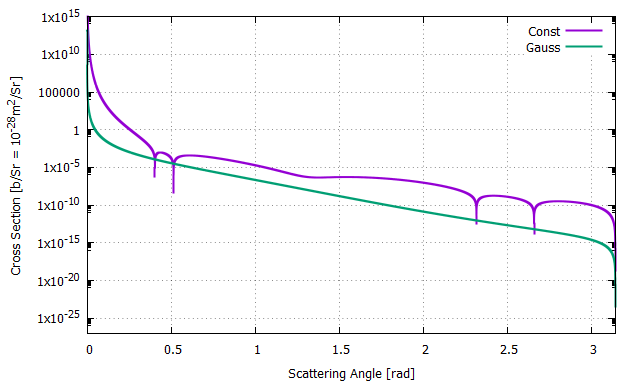
\includegraphics[bb = 120 0 500 430, width=11.0cm]{tamu_fig03.png}
            \caption{微分断面積の散乱角依存性}
        \end{figure}
    \newpage
    \section{}
        \subsection{}
        \begin{description}
            \item[(i). s process]
            重い原子核を合成するためには、陽子の増加に伴うCoulomb力による反発をキャンセルする必要が出てくるため、陽子よりも中性子を多く取り込むことによって$n-n$間での引力を稼ごうとする。つまり重い原子核の合成には中性子が必要になる。この中性子の捕獲に要する時間が原子核の$\beta$崩壊の寿命よりも長いか或いは短いかというのがsプロセスとrプロセスの違いである。\\
             中性子捕獲が起こるためには中性子が存在していなくてはならない。燃焼している恒星内部において中性子は
            \begin{eqnarray}
                &&{}^{22}_{10}{\rm{Ne}}+\alpha\to{}^{25}_{12}{\rm{Mg}}+{\rm{n}}-0.48{\rm{MeV}}\\
                &&{}^{12}_{6}{\rm{C}}+\alpha\to{}^{16}_{8}{\rm{O}}+{\rm{n}}-0.91{\rm{MeV}}
            \end{eqnarray}
            といった反応によって合成される。このような反応によって生じた中性子を捕獲することによって、中性子過剰核を生じ、$\beta$崩壊を生じる。
            \begin{eqnarray}
                &&\left(Z,A\right)+{\rm{n}}\to\left(Z,A+1\right)+\gamma\\
                &&\left(Z,A+1\right)\to\left(Z+1,A+1\right)+e^-+\bar{\nu}_e
            \end{eqnarray}
            この$\beta$崩壊によって、形成される中性子過剰な同位体は安定な同重体になる。こうして、核図表において安定な原子核に沿った線であるHeisenbergの谷に沿ってより重い元素が合成されていく。この過程においては最も重い核種として${}^{209}{\rm{Bi}}$が生成されるが、これは不安定核であるため$\beta$崩壊及び$\alpha$崩壊によって${}^{206}{\rm{Pb}}$になる。したがって、この過程で生成される最も重い原子核は${}^{206}{\rm{Pb}}$となる。\\
            \item[(ii). r process]
             前述のsプロセスでは${}^{206}{\rm{Pb}}$までの核種しか合成することはできない。もし、合成された不安定核が崩壊するよりも早く中性子を吸収することができれば、より重い原子核も合成することが可能になる。そのようなことが起こるためには$10^{23}\,{\rm{/cm^3}}$以上という非常に高い密度で中性子が存在している必要がある。このような状況は恒星内部では起こせないが、超新星爆発の際には起こると予想されている。この時には中性子のフラックスは$10^{32}\,{\rm{m^{-2}\cdot{s}^{-2}}}$にもなると考えられ、上記の条件が満たされるであろうと予想されるためである。このような反応過程は前述のsプロセスと比較して非常に短い時間スケールで起こる反応と考えられる。そのためr(rapid)プロセスと呼ばれる。
        \end{description}
        \textbf{問5(1)の参考文献・URL}
        \begin{description}
            \item[1.]B.Povh, K.Rith, C.Scholz: 素粒子・原子核物理入門 (丸善出版)
            \item[2.]熊野俊三: KEK物理学シリーズ2 原子核物理学 (共立出版)
        \end{description}
        \newpage
        \setcounter{subsection}{2}
        \subsection{}
         重い元素の合成の証拠とされているのは、「キロノバ」の観測データである。キロノバとは、中性子合体の際にrプロセスによって合成された重い原子核の崩壊に伴い可視光や赤外線といった電磁波を放出する現象のことである。各原子核のエネルギー準位の構造からどのような振動数の電磁波が放出されるのかを予想することができる。特にランタノイド族では主として赤外線が、それよりも軽い元素では可視光など比較的振動数の高い電磁波がみられる。光の色は振動数が低いものほど赤く、高いものほど青く見えることから、前者を「赤いキロノバ」、対して後者を「青いキロノバ」という。このようなことと検出される電磁波のスペクトルを調べることによって、その際にどのような元素が合成されていたのかを知ることができる。実際に観測されたデータからは、
        \begin{description}
            \item ・超新星爆発とは全く異なるものであった
            \item ・約0.03太陽質量以上の物質が放出されている
            \item ・観測された放射では赤外線が卓越していた
            \item ・最初の数日間は可視光も見られた(ランタノイド以外の放出も多いことの示唆)
        \end{description}
        といった事実が得られた。特に物質の放出量に関して、中性子星合体でいつも約0.03太陽質量の重元素が放出されているならば、銀河系でのrプロセスでの元素の量を説明するのに十分な量になると考えられている。\\
        \textbf{問5(2)の参考URL}\\
        いずれも2019年8月8日閲覧
        \begin{description}
            \item[1.] 「原子核物理学II」(萩野浩一先生担当)の講義資料(\url{http://www.nucl.phys.tohoku.ac.jp/~hagino/lectures/nuclphys2/notes19-7.pdf})
            \item[2.] \url{http://www.asj.or.jp/geppou/archive_open/2018_111_02/111-2_86.pdf}
        \end{description}
\end{document}


%https://tohoku.repo.nii.ac.jp/?action=repository_uri&item_id=50540&file_id=18&file_no=1 (メスバウアー効果の概念とその応用例)
%https://tenkyo.net/kaiho/pdf/2002_05/2002-05-09.pdf 
%http://www.icrr.u-tokyo.ac.jp/ss/2014data/lecture/ohashi.pdf
%\textbf{参考文献}
%\begin{description}
%    \item[1.]八木浩輔: 基礎物理科学シリーズ4 原子核物理学 (朝倉書店)
%    \item[2.]中嶋貞雄、豊沢豊、阿部龍蔵: 現代物理学の基礎7 物性II 素励起の物理 (岩波書店)
%\end{description}